\chapter{Material e Métodos ou Desenvolvimento do Projeto}
\label{Material}


% % % % % % % % % % % % % % % % % % % % % % % % % % % % % % % % % % % % % % % % % % % % % % % % % % %
\section{Material}
\par Com a intenção de solucionar um problema do mundo real e facilitar vidas no que diz respeito à acessibilidade, de maneira a realmente otimizar de alguma forma o mundo das pessoas envolvidas, surgiu a idéia de desenvolver um sistema para que quem tenha deficiência auditiva possa se comunicar com outros que desconhecem a linguagem para surdos mudos, já que esta é pouco difundida e ensinada, trazendo desta forma melhorias para os deficientes em sua desenvoltura pessoal, vida profissional e educação, além de incentivar a aprendizagem da Libras. 

\par O Projeto base tem por objetivo estruturar e desenvolver um sistema de interpretação dos números do alfabeto da Libras de 0 a 7.

\par Sendo assim, o Projeto principal consiste em um aplicativo Android conectado a um sistema embarcado em uma Raspberry Pi com Raspian rodando em rede e com comunicação Web para um website para treinamento de rotinas da Linguagem. Ou seja, generalizando a divisão do projeto, tem-se os seguintes materiais envolvidos:

\begin{itemize}
	\item Android Studio: Para a criação do aplicativo, o qual processa as imagens da câmera do Smartphone para transferi-lás à Raspberry e aparecendo conocmitantemente no website implementado 

	\item Raspberry Pi: Pequeno microcomputador, embarcado com uma distribuição Linux e programado para as necessidades do projeto de interpretar a linguagem de Libras.
	\item Raspian: Distrubuição variante do Debian do Linux baseada na arquitetura ARM do hardware da Raspberry Pi.
	\item Python: Linguagem de programação interpretada de alto nível utilizada durante toda execução do projeto, tanto para rotinas internas de classificação, quanto para criação do website.
    \item Flask: Framework pequena e poderosa para Python utilizada na criação do sistema Web.
	\item OpenCV: Significando Open Source Computer Vision Library, é uma biblioteca multiplataforma utilizada no aplicativo Android afim de processar as imagens obtidas na câmera.
	
	\item Materilize: Framework FRont-End com uma interface gráfica mais agradável, utilizada em nosso sistema web de treinamento de símbolos.
	\item MongoDB: Modelo de banco de dados NoSQL que facilita sua crianção, servindo como armazenamento das imagens dos símbolos das Libras para posteriores comparações e classificações.
    
\end{itemize}

\par O sistema e suas comunicações, em resumo, funcionam da seguinte maneira: O aplicativo Android é responsável por adquirir a imagem via câmera do \textit{Smartphone}, conta em sua implementação com OpenCV (Open Source Computer Vision Library) para interpretar as imagens, detectando bordas, pele e face, envia então essas imagens de modo simultâneo para o sistema rodando na Raspiberry


% % % % % % % % % % % % % % % % % % % % % % % % % % % % % % % % % % % % % % % % % % % % % % % % % % %
\section{Métodos}

\par A metodologia utilizada para realizar este trabalho baseia-se nas metodologias utilizadas em~\cite{Barros},~\cite{Yeo} e~\cite{Chen}. Basicamente o processo se divide conforme mostra a figura~\ref{fig:processo}.

\begin{figure}[H]
	\centering
	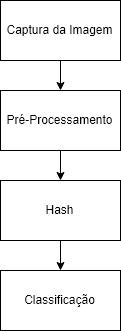
\includegraphics[width=0.2\textwidth]{./Resources/procedimento.png}
	\caption{Método utilizado.}
	\label{fig:processo}
\end{figure}

\subsection{Captura da Imagem}

\par A captura da imagem é feita pela câmera do aparelho Android. Não foi imposta nenhuma restrição quanto às características da câmera para este projeto.

\subsection{Pré-Processamento}

\par O pré-processamento é realizado com auxílio da biblioteca \textit{OpenCV} e consiste em tratar a imagem capturada pela câmera de modo isolar as características desejadas (neste caso, busca-se isolar a região das mãos).

\par O processo de pré-processamento é mostrado na figura~\ref{fig:pre_proc}. São realizadas 3 etapas de maneira independente:

\begin{itemize}
	\item Detecção de bordas: feita por meio da função \textit{Imgproc.Canny}. 
	\item Detecção de face: utiliza o \textit{CascadeClassifier} da biblioteca \textit{OpenCV} para fazer a detecção da região quadrada que contém uma face. Esta região é então preenchida (preto) de modo a eliminar a face da imagem.
	\item Detecção de pele: 
\end{itemize}

\begin{figure}[H]
	\centering
	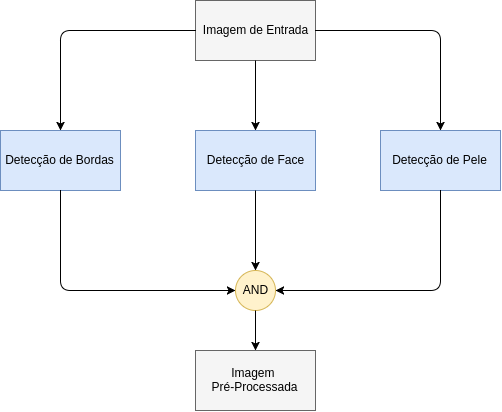
\includegraphics[width=0.7\textwidth]{./Resources/pre_processamento.png}
	\caption{Pré-Processamento aplicado.}
	\label{fig:pre_proc}
\end{figure}

